%--
%  Vistas: está sería la parte principal del TP. Acá irían los diagramas y los
%  escenarios representativos de uso. No necesariamente tiene que ser una gran
%  sección, sino que pueden partirla por funcionalidades y a su vez por tipo de
%  vista o de la forma que crean más pertinente. Esta sección NO DEBE SER una
%  simple seguidilla de figuras sueltas. Debe estar acompañada de tantas
%  explicaciones como sean necesarias para que se aprecie un hilo conductor.
%--
\section{Vistas}

  %--
  %-- Diagrama de Contexto
  %--
  \subsection{Diagrama de Contexto}
    
    %--
    %-- Acciones Básicas
    %--
    \subsubsection{Acciones básicas}
    \begin{figure}[H]
      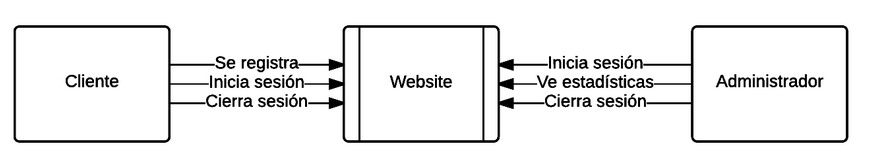
\includegraphics[width=\linewidth]{images/acciones-basicas.png}
    \end{figure}
    \fixme[Agregar el texto que describe este gráfico]

    %--
    %-- Cliente recibe pedido
    %--
    \clearpage
    \subsubsection{Cliente recibe pedido}
    \begin{figure}[H]
      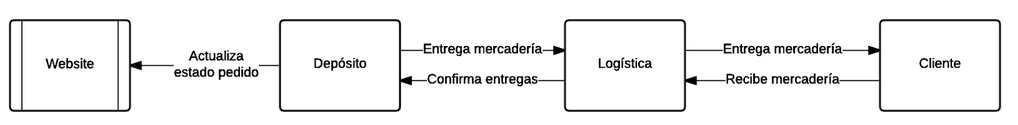
\includegraphics[width=\linewidth]{images/cliente-recibe-pedido.png}
    \end{figure}
    \fixme[Agregar el texto que describe este gráfico]

    %--
    %-- Cliente no recibe pedido
    %--
    \clearpage
    \subsubsection{Cliente no recibe pedido}
    \begin{figure}[H]
      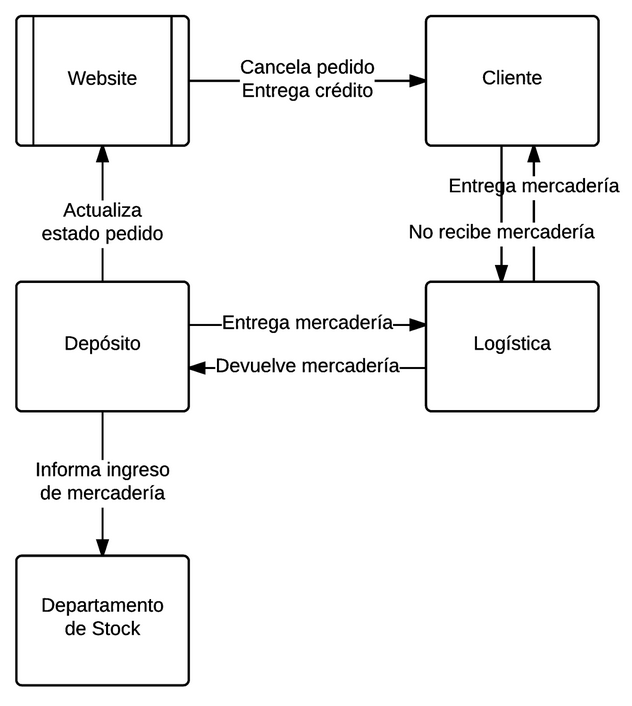
\includegraphics[width=\linewidth]{images/cliente-no-recibe-pedido.png}
    \end{figure}
    \fixme[Agregar el texto que describe este gráfico]

    %--
    %-- Reposición de stock en depósito
    %--
    \clearpage
    \subsubsection{Reposición de stock en depósito}
    \begin{figure}[H]
      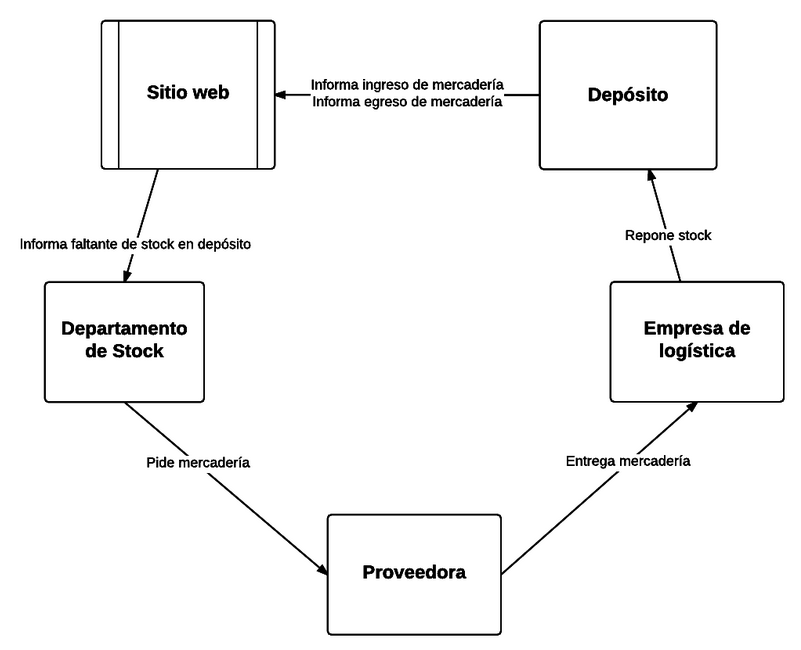
\includegraphics[width=\linewidth]{images/reposicion-stock-deposito.png}
    \end{figure}
    \fixme[Agregar el texto que describe este gráfico]

    %--
    %-- Reposición de stock en sucursal
    %--
    \clearpage
    \subsubsection{Reposición de stock en sucursal}
    \begin{figure}[H]
      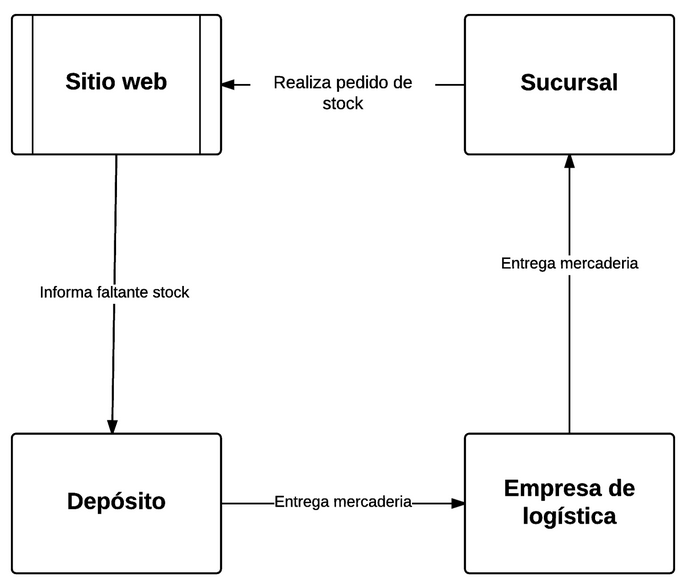
\includegraphics[width=\linewidth]{images/reposicion-stock-sucursal.png}
    \end{figure}
    \fixme[Agregar el texto que describe este gráfico]

    %--
    %-- Solicitud de pedido por cliente
    %--
    \clearpage
    \subsubsection{Solicitud de pedido por cliente}
    \begin{figure}[H]
      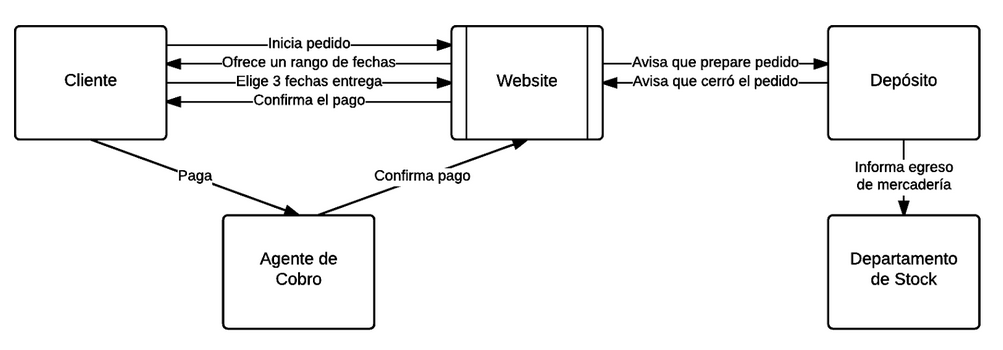
\includegraphics[width=\linewidth]{images/solicitud-de-pedido-por-cliente.png}
    \end{figure}
    \fixme[Agregar el texto que describe este gráfico]

  %--
  %-- Modelo de Objetivos
  %--
  \clearpage
  \subsection{Modelo de Objetivos}
  \fixme
  
  %--
  %-- Escenarios de uso
  %--  
  \newpage
  \subsection{Escenarios representativos de uso}
    
    %-- Escenario 1
    \subsubsection{Registro, compra y pago online}

    Un usuario entra por primera vez al sitio, y se registra. Luego inicia sesión y el sistema le da la posibilidad de hacer una compra online. Una vez seleccionado los productos deseados y terminado de hacer el pedido, el usuario debe elegir la fecha de entrega. Para ello el sistema hace una consulta a la Empresa de Logística, para ver cuándo puede hacer la entrega. 
    
    Una vez elegida la fecha, se le da la opción de pago. De acuerdo al rating del usuario, puede ser contra entrega o también online. Si el usuario decide utilizar la segunda, entonces el sitio le muestra la pantalla de pago del Agente de Cobro correspondiente. Si el pago es satisfactorio, el Agente de Cobro se lo confirma al sitio, y este le solicita al Depósito que lo prepare. Una vez cerrado el pedido, el Depósito le inforuo”. Logística pueda lo busca para entregárselo al cliente. 
    
    Si el usuario lo recibe satisfactoriamente, entonces Logística lo informa a Depósito, quién actualiza otra vez el estado del pedido en el sitio a “Entregado”. 

    %-- Escenario 2
    %\subsubsection{Nombre del escenario}

    \fixme